\documentclass{article}

\usepackage{lipsum}
\usepackage[margin=2cm, left=2cm, includefoot]{geometry}
\usepackage{graphicx}
\usepackage{float}
\usepackage{hyperref}

% Header and footer
\usepackage{fancyhdr}
\pagestyle{fancy}

\rhead{}
\lhead{}
\fancyfoot{}
\fancyfoot[R]{\thepage}
\renewcommand{\headrulewidth}{0pt}
\renewcommand{\footrulewidth}{0pt}
%

\begin{document}

\begin{titlepage}
	\begin{center}
		\line(1,0){300}\\
		[6mm]
		\huge{\bfseries PROJECT TENDER}\\
		[2mm]
		\line(1,0){200}\\
		[5mm]
		\large\textbf{PROJECT:}\\\textsc{Network Visualizations Interface for Large Scale Networks}\\
		[3mm]
		\large\textbf{CLIENT:}\\\textsc{Ivan du Toit}\\
		[3mm]
		\large \textbf{TEAM:}\\\textsc{Funge}\\
		\line(1,0){350}\\
		[5mm]
		\large \textbf{Team Members:}\\
		[3mm]
		\large Gian Paolo Buffo - 14446619\\
		\large Matthew Botha - 14214742\\
		\large Matthias Harvey - 14027021\\
        \large Dillon Heins - 14035538\\[3mm]
		\begin{figure}[H]
			\centering
			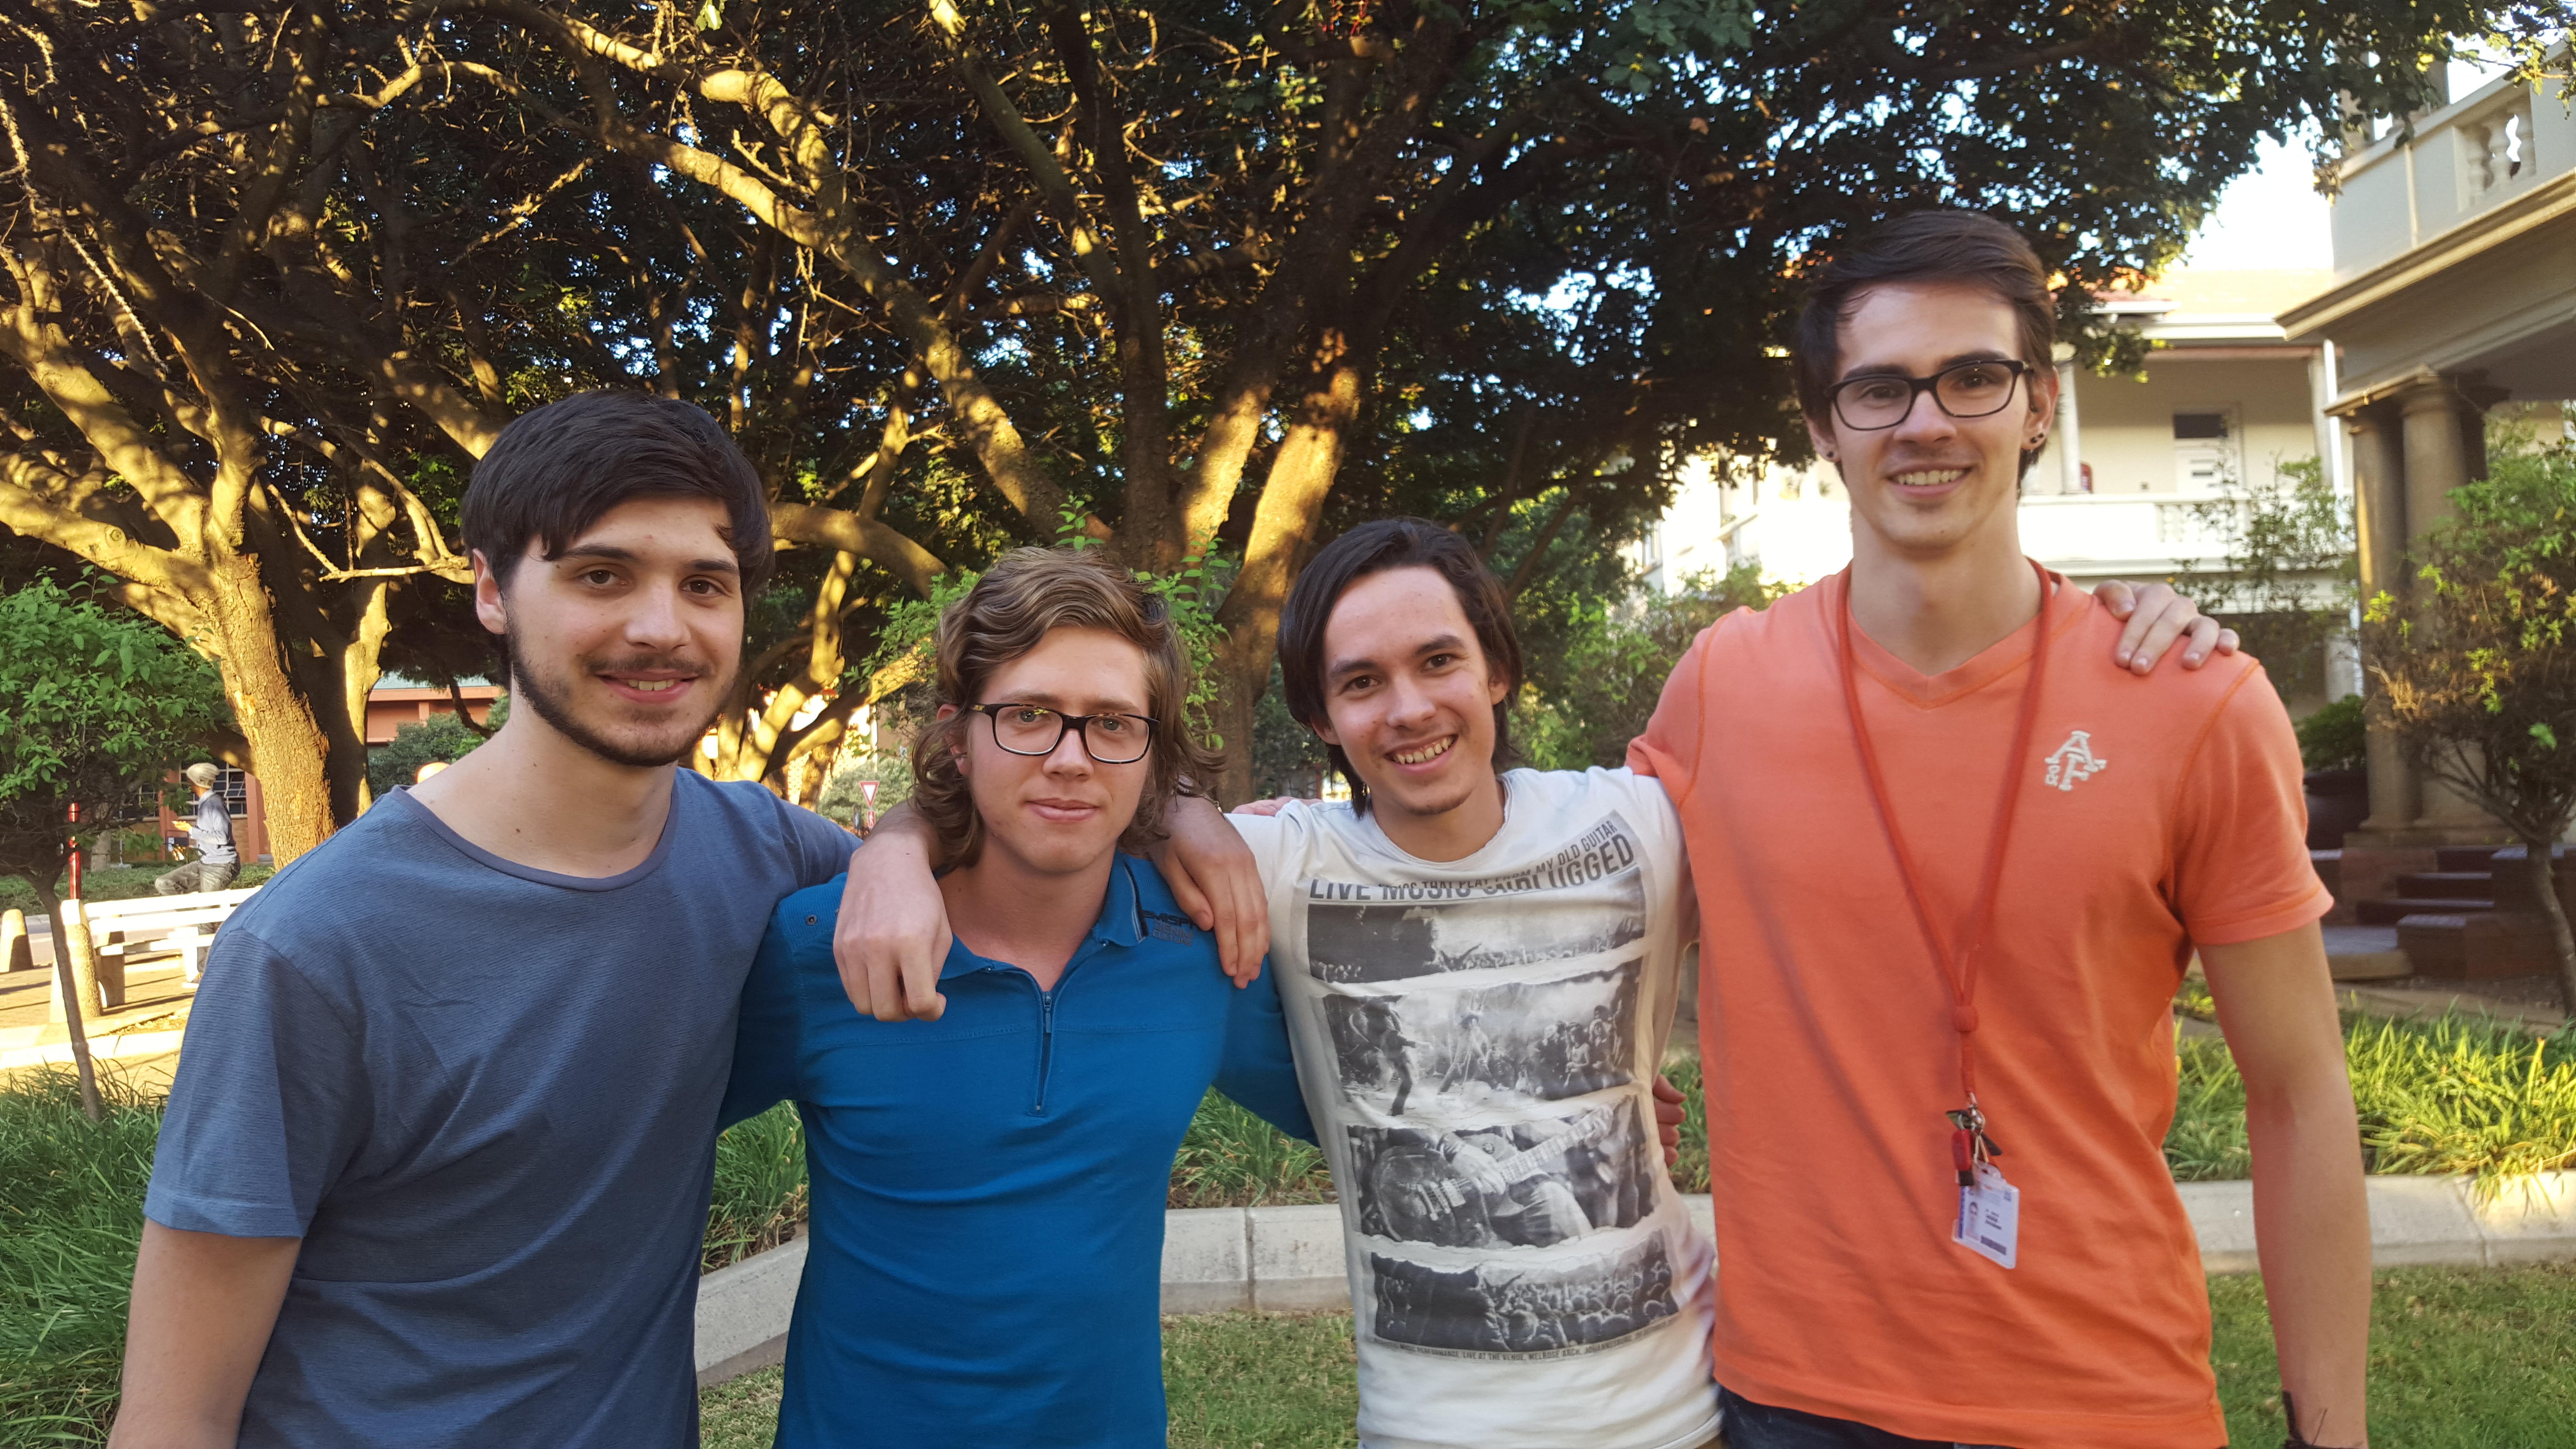
\includegraphics[width=0.8\textwidth]{../teamPhoto.jpg}
			\caption{Matthew Botha, Matthias Harvey, Gian Paolo Buffo, Dillon Heins}
		\end{figure}
    \end{center}

	\vspace{7mm}

    \begin{flushright}
        \textsc{\large Department of Computer Science\\
        University of Pretoria\\
        01 May 2016\\}
    \end{flushright}
\end{titlepage}

\section{The Team}
	\subsection{Dillon Heins - 14035538}
	\subsubsection{Contact}
		\begin{itemize}
			\item \href{https://za.linkedin.com/in/dillon-heins-54275810a}{LinkedIn - Dillon Heins}
			\item \href{mailto:dillonheins@gmail.com}{dillonheins@gmail.com}	
		\end{itemize}
	\subsubsection{Photo}
		\begin{figure}[H]
			\centering
			\includegraphics[width=0.7\textwidth]{../dillon.jpg}
			\caption{Dillon Heins}
		\end{figure}
	\subsubsection{Interests}
		\begin{itemize}
			\item Algorithms and data structures
			\item Computer networks
			\item Computer graphics
			\item Computer security
			\item Game development and design
		\end{itemize}
	\subsubsection{Technical Skills}
		\begin{itemize}
			\item Strong programming, algorithmic and data structure skills
			\item Proficient in the use of multimedia i.e. the combining of computer science, visual design and multimedia to create a complete and coherent product
			\item Adept in the learning and application of newly acquired skills
			\item Proficient in the programming and understanding of networked software
		\end{itemize}
	\subsubsection{Past Experience \& Achievements}
		\begin{itemize}
			\item \textbf{Past Experience}
			\begin{itemize}
				\item Web Developer for Ms. Vreda Pieterse (Software engineering lecturer)
				\begin{itemize}
					\item University of Pretoria
					\item July 2014 - Present
				\end{itemize}
				\item Teaching Assistant
				\begin{itemize}
					\item University of Pretoria
					\item February 2016 - Present
				\end{itemize}
			\end{itemize}
			
			\item \textbf{Achievements}
			\begin{itemize}
				\item
			\end{itemize}
		\end{itemize}
		
	\subsubsection{Non-technical Skills}
	\subsubsection{Motivation for Choosing Project}

\cleardoublepage
    
\section{Project Execution}

\end{document}
